\documentclass{scrartcl}
\usepackage[ngerman]{babel} % default Sprache für alles (Datum usw.)
\usepackage[affil-it]{authblk}
\usepackage{setspace} % Zeilenabstand
\usepackage{csquotes} % um ,,hello" zu benutzen
\usepackage[sorting=none]{biblatex} 
\usepackage[most]{tcolorbox} % Codeblocks
\usepackage{graphicx}
\usepackage[bottom]{footmisc}
\usepackage{booktabs}
\DefineBibliographyStrings{ngerman}{ % u.a. -> et al.
   andothers = {et al\adddot}
}
\definecolor{gray}{rgb}{0.94, 0.94, 0.95}
\setlength{\parindent}{0pt} % Sets the paragraph indent to 0

\addbibresource{references.bib}

\begin{document}

\begin{titlepage}

   \subject{Literatur-Seminar-Arbeit}
   \title{Vorhersagen von Verkehrsunfällen mithilfe künstlicher neuronaler Netze}
   \author{Erik Rohr}
   \affil{Fachbereich Informatik (02) - Hochschule Bonn-Rhein-Sieg}
   \publishers{\parbox[b][12cm]{\textwidth}{\centering Betreuerin: Doerthe Vieten}}
   \date{\today}

   \maketitle

\end{titlepage}

\newpage
\onehalfspacing

\section*{Abstrakt}
$\ll$ Kurz beschreiben $\gg$

\newpage
\tableofcontents
\newpage

\section{Einleitung}

Jedes Jahr sterben weltweit ca. 1,19 Millionen Menschen in Verkehrsunfällen
(RTA, engl.: \enquote{road traffic accident}) \cite{who}.
Eine umfassende Analyse vorliegender Verkehrsdaten im Hinblick auf potentielle
Bedrohungen kann dazu beitragen, Baumaßnahmen unfallminimierend zu gestalten.
\medskip \\
Vorangehende Analysen von Verkehrsdaten, die eine Vielzahl an \enquote{Machine Learning}
-Modelle nutzten, haben ergeben, dass eine Vielzahl an Faktoren existieren,
die das Risiko auf RTA erhöhen, wie Wetterbedingungen, Straßenkonditionen,
Zustand des Fahrers, Lichtverhältnisse, Tageszeit und die Verkehrsdichte \cite{ml, predict}.
\enquote{Machine Learning}-Modelle (ML) sind darauf ausgelegt, nicht anhand von
spezifischen Anweisungen, sondern allein durch das Erkennen von Mustern und
Abhängigkeiten mithilfe komplexer Funktionen \cite{predict} in Daten Erkenntnisse
zu ziehen und Entscheidungen sowie Vorhersagen treffen zu können \cite{sap}.
\medskip \\
Unter den ML-Modellen werden künstliche neuronale Netze (KNN) für diesen
Anwendungsfall bevorzugt, da diese keine zugrundeliegenden Beziehungen
zwischen den Eingangsvariablen benötigen und darauf ausgelegt sind,
mit historischen Daten Aussagen über die Zukunft treffen zu können
\cite{predict}.
\medskip \\
In dieser Arbeit wird eine systematische Literaturrecherche (SLR) zur Vorhersage
von RTAs mithilfe KNNs dargestellt. Die Ergebnisse werden im Hinblick auf deren
Mehrwert in der Minimierung von Straßenverkehrsunfällen durch unsichere
Planung der Architektur untersucht und eingeordnet.

\subsection{Theorie}

\subsubsection{Künstliche neuronale Netze (KNN)}
Künstliche neuronale Netze (KNN) sind ein Teilbereich der ML-Modelle. Sie können
Entscheidungen auf ähnlicher Art und Weise treffen, wie das menschliche Gehirn \cite{ibm}.
Das Modell besteht aus einer Vielzahl von Schichten mit unterschiedlich vielen
Knoten. Diese Knoten sind mit anderen Knoten aus den benachbarten Schichten verbunden
und besitzen sogenannte \enquote{weights} und \enquote{bias} \cite{ibm}.
Eingabedaten werden von der \enquote{input layer} (Deutsch: \enquote{Eingangsschicht})
entlang aller hidden layer (Deutsch: \enquote{verborgene Schicht}) durchgereicht,
verarbeitet und schließlich in der \enquote{output layer}
(Deutsch: \enquote{Ausgangsschicht}) aggregiert ausgegeben \cite{ibm}.
\medskip \\
Zur Konfigurierung von KNN können unter anderem die Anzahl der Schichten,
die Optimierungsverfahren (engl.: \enquote{optimizers}), die
Aktivierungsfunktion (engl.: \enquote{activation function}) und die
Verlustsfunktion (engl.: \enquote{loss function}) frei gewählt werden
\cite{actopt}.
\medskip \\
Ein Optimierungsverfahren ist eine Funktion oder ein Algorithmus, welches
Parameter der Knoten wie die Gewichte und die Lernrate (engl.: \enquote{learning rate})
anpasst, um den Verlust zu minimieren, die Genauigkeit zu maximieren und
die benötigte Trainingszeit exponentiell zu reduzieren \cite{actopt}.
Beispiele für solche Optimierungsverfahren sind der \enquote{gradient descent},
\enquote{RMS prop (Root Mean Square)} und \enquote{adam's optimizer} \cite{actopt}.
\smallskip \\
Die Aktivierungsfunktion entscheidet, wie der kalkulierte Ausgangswert
eines Knotens zu interpretieren ist. Dies fügt dem Netz eine Nicht-Linearität
hinzu \cite{actopt}. Somit können die verborgenen Schichten jeweils für
andere Bereiche der Interpretation der Daten stehen. Linearität würde auf
der anderen Seite bedeuten, dass das Netz in eine Funktion zusammengefasst
werden könnte \cite{actopt}. Beispiele sind die binäre \enquote{step function},
die Sigmoid-Funktion und die \enquote{RELU}-Funktion \cite{actopt}.
\smallskip \\
Eine Verlustsfunktion misst, wie genau das KNN den Datensatz modelliert, indem
es den vorliegenden Verlust (engl.: \enquote{loss}) berechnet \cite{actopt}.
Gängige Funktionen sind die \enquote{Mean Squared Error}-Funktion und die
\enquote{Binary Cross Entropy}-Funktion \cite{actopt}.

\subsection{Aktuelle Forschungslage}

\subsubsection{Banerjee et al.}
Eine Vielzahl an Klassifizierern (engl.: \enquote{classifiers}) sind mit
KNN-Modellen bezüglich Vorhersage der Mortalität in RTAs verglichen worden.
Darunter gehören
Random Forest, Support Vector Machine, K-Nearest Neighbor Classifier,
AdaBoost Classifier, XGBoost Classifier. Hierbei hat das KNN mit 7
\enquote{hidden layer}, 1 \enquote{input layer}, Adams Optimizer und einer
\enquote{dropout class} in der Eingangsschicht die beste Genauigkeit von 84,36\%
erzielt \cite{akt1}.

\subsubsection{Maurya et al.}
Vorhersehen von Kraftfahrzeuggeschwindigkeiten dienen als Basis für ein
fortgeschrittenes Verkehrsmanagementsystem \cite{akt2}. Hierbei wurden
Lineare Regression, \enquote{random forest}-Regression, \enquote{Decision Tree} und
ein KNN miteinander Vergleichen uns eine \enquote{Performance Analyse} durchgeführt.
KNN und die \enquote{random forest}-Regression haben mit einem
\enquote{R squared}-Wert \footnote{Bestimmtheitsmaß.
   Stellt die Anpassungsgüte einer Regression dar \cite{rsquared}}
von jeweils 0,9301 und 0,9642 das beste Fitting erzielt \cite{akt2}.

\subsubsection{Zohra et al.}
Anhand den Datensätzen aus \enquote{US Accidents (2016-2023)} wurden ein KNN,
ein Random Forest Klassifizierer und eine logistische Regression trainiert und
getestet. Hier wurden jeweils Genauigkeitswerte von 81,1\%, 90,7\% und 87,03\%
erreicht \cite{akt3}.


\section{Methodik}
Im Folgenden wird die Vorgehensweise bei der Literaturrecherche beschrieben.
Die Vorgehensweise orientert sich an der PRISMA-Leitlinie (Preferred Reporting
Items for Systematic Reviews and Meta-Analyses). PRISMA hat sich ursprünglich
als effektiver Vorreiter bzgl. SLR im medizinischen Sektor etabliert, mit dem
Fachkräfte auf dem aktuellen Stand der Wissenschaft bleiben und bestehende
Vorschriften aktualisiert werden \cite{prisma}. Entnehmend der zahlreichen
SLR-Veröffentlichungen in Bereichen der Informatik (siehe Datenbanken ACM/IEEE),
hat sich PRISMA als hilfreiches Mittel zur SLR auch in anderen
Wissenschaftsbereichen bewiesen.

\subsection{Die PRISMA-Leitlinie}
PRISMA beinhaltet eine aus 27 Stichpunkten bestehende \enquote{Checkliste}
und ein 4-phasiges Fluss-Diagramm \cite{prisma}. Da diese allerdings ursprünglich
für die Medizin entwickelt wurden, werden jene auf die angepasst Informatik
für die Basis der SLR verwendet.  Mithilfe dieser Elemente kann sowohl Literatur
systematisch für die Aufnahme in einer SLR auf Eignung geprüft als auch der
Prozess erleichtert und standardisiert werden.

Zunächst werden Forschungsfragen aufgestellt, die im Laufe der Recherche beantwortet
werden sollen. Im Anschluss wird dann die Literatur anhand der ausgewählten
Such-Strategie ausgewählt. Die gesammelte Literatur wird dann durch Ein- und
Ausschlusskriterien gefiltert und auf Eignung für die SLR durch die Checkliste geprüft.
Schließlich werden aus der eingeschlossenen Literatur qualitative und quantitative
Daten extrahiert, mit anderer Literatur verglichen und in der eigentlichen
Literaturanalyse zusammengetragen.

\subsection{In- und Exklusionskriterien}
Um gezielt die Potenz künstlicher neuronaler Netze für die Verkehrsanalyse zu
untersuchen, sind gezielt Ein- und Ausschlusskriterien gewählt worden. Somit
wird die Anzahl der aus der Suche ergebenen Artikel reduziert und verschafft
einen besseren Überblick.

Die für diese Arbeit relevanten Artikel sind auf solche beschränkt worden, die
\begin{enumerate}
   \item{eine Verkehrsdatenanalyse untersuchen und die Daten mit einer KNN auswerten,}
   \item{ggf. einen quantitativen Vergleich verschiedener ML-Modelle durchführen oder}
   \item{quantitative Merkmale der KNN aufzählen.}
\end{enumerate}
Zu letzterem Punkt gehören Merkmale wie gewählte Netztopologie, Anzahl der Schichten,
Anzahl der Knoten pro Schicht, gewähltes Optimierungsverfahren, die gewählte
Aktivierungsfunktion Genauigkeit und Eingangsvariablen.

\subsection{Prozess der Recherche}

Für die Literaturrecherche sind die Datenbanken ACM Digital Library und die
IEEE Explore verwendet worden, da diese überwiegend Artikel in der Informatik
veröffentlicht haben.
Hierbei wurden die folgenden Suchstrings verwendet:

\begin{tcolorbox}[
      enhanced,
      attach boxed title to top left,
      colback=gray!20,
      colframe=gray,
      colbacktitle=gray,
      title=ACM Digital Library,
      fonttitle=\bfseries\color{black},
      boxed title style={size=small, colframe=gray, sharp corners},
      sharp corners
   ]
   [All: "neural network?"]
   AND [
         [All: "traffic flow"]
         OR [All: "traffic control"]
         OR [All: \dq accident"]
      ]
   AND [E-Publication Date: (01/01/2023 TO 12/31/2024)]
\end{tcolorbox}

\begin{tcolorbox}[
      enhanced,
      attach boxed title to top left,
      colback=gray!20,
      colframe=gray,
      colbacktitle=gray,
      title=IEEE Explore,
      fonttitle=\bfseries\color{black},
      boxed title style={size=small, colframe=gray, sharp corners},
      sharp corners
   ]
   (\dq All Metadata\dq: \dq artificial neural network?")
   AND (\dq All Metadata":"traffic")
   AND (\dq All Metadata":"control\dq\space
   OR \dq All Metadata":\dq accident")
\end{tcolorbox}

Bei der \enquote{IEEE-Explore}-Datenbank wurde als Zeitraum-Filter der 01.01.2023
bis zum 31.12.2024 gewählt, da dieser nicht in den Such-String mit eingebunden
werden konnte.  Zusätzlich ist die Suche auf den Inhaltstyp
\enquote{Research Article} und die Verfügbarkeit \enquote{Open Access}
begrenzt worden, soweit von den Einstellungen beider Datenbanken möglich.
\medskip \\
Die zusammengetragenen Artikel wurden im Anschluss mithilfe des PRISMA 
Fluss-Diagramms \cite{prisma} auf Eignung überprüft (Abb. \ref{abb1}) und in einer Tabelle
zusammengefasst (Tab. \ref{tab1}).

\begin{figure}[h]
   \centering
   \caption{SLR nach PRISMA}
   \label{abb1}
   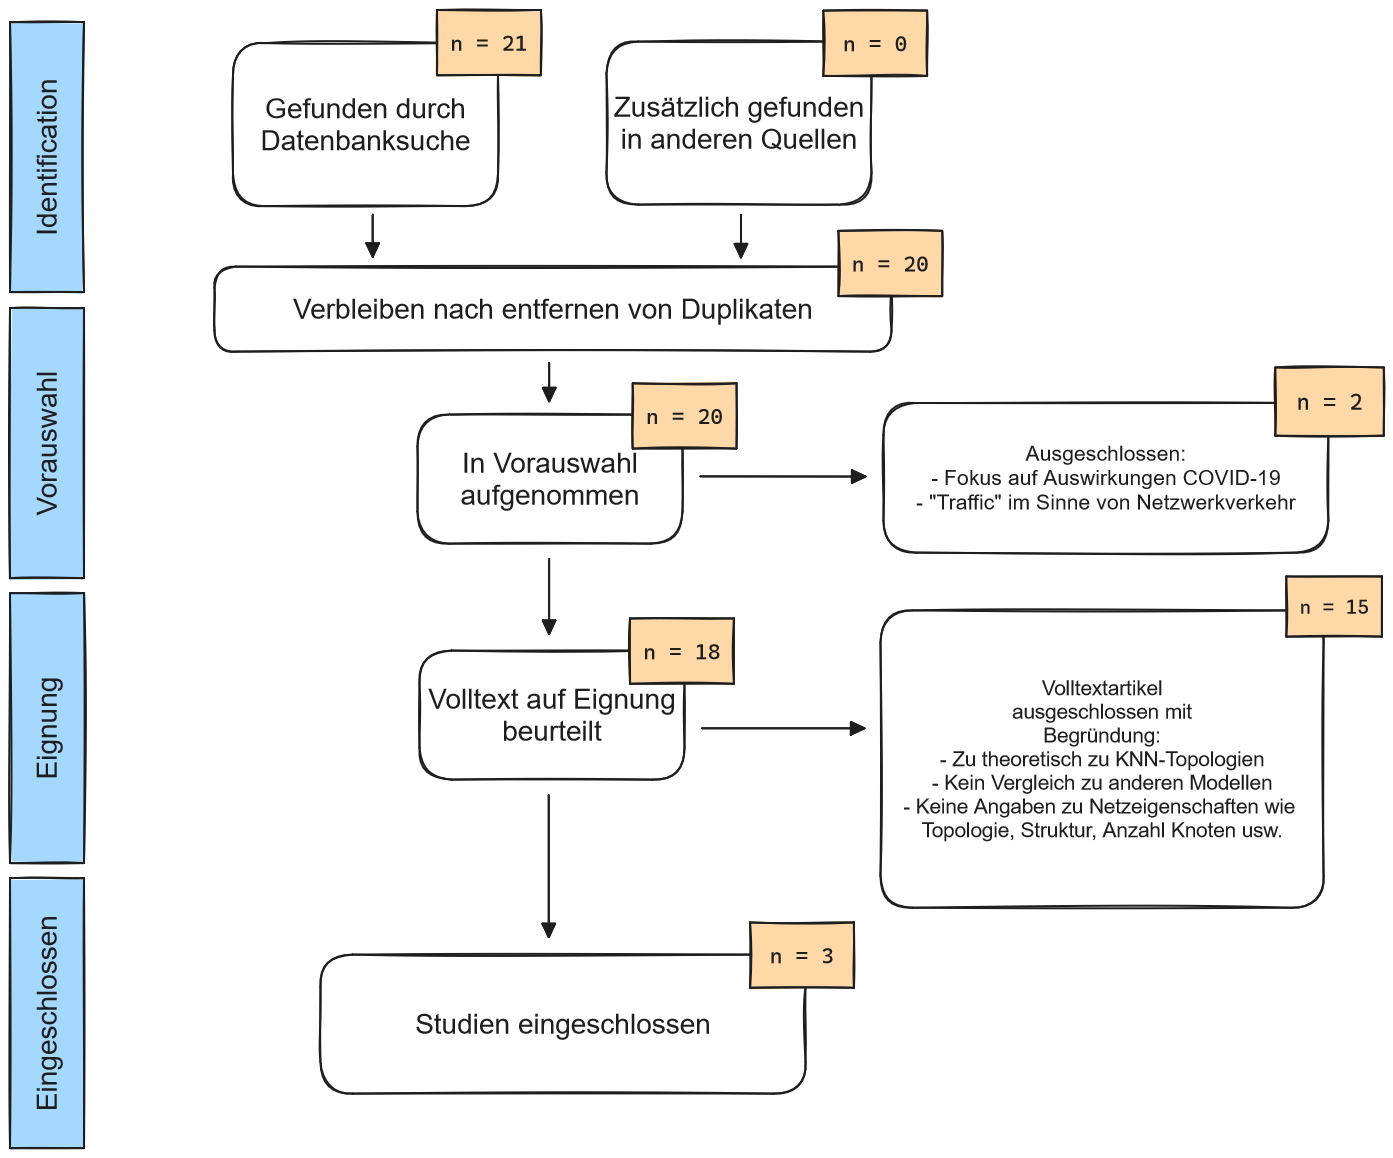
\includegraphics[scale=0.28]{Bilder/prisma-exported.png}
\end{figure}

\section{Ergebnisse}

\begin{table}[h!]
   \centering
   \caption{Ergebnisse der Literaturrecherche}
   \label{tab1}
   \begin{tabular}{lccc} \toprule
      Autoren               & Qian et al. \cite{qian} & Das et al.  \cite{das} & Bao et al. \cite{bao} \\ \midrule
      Topologie             & BPNN                    & FF                     & BPNN                  \\
      Aktivierungsfunktion  & Softmax                 & Softmax                & Sigmoid               \\
      Verlustsfunktion      & Cross-Entropy           & Cross-Entropy          & o.A.                  \\
      Verborgene Knoten     & $3$                     & o.A.                   & $388$; $300 + 88$     \\
      Lernrate              & $0.01$                  & o.A.                   & $0.005$               \\
      Optimierungsverfahren & Gradient Descent        & Adam Optimizer         & o.A.                  \\
      Genauigkeit           & $78.56 \%$              & $94.62 \%$             & $76.1 \%$             \\
      Eingabevariablen      &                         &                        &                       \\ \bottomrule
   \end{tabular}
\end{table}

\section{Diskussion und Fazit}

\subsection{Diskussion}

$\ll$ Forschungsfrage aufgreifen und beantworten $\gg$

\subsection{Limitationen}

$\ll$ Grenzen dieser Arbeit auflisten $\gg$

\subsection{Fazit}

$\ll$ Zusammenfassen $\gg$

\subsection{Ausblick auf zukünftige Forschung}

$\ll$ Selbsterklärend $\gg$

\printbibliography
\listoffigures
\listoftables

\end{document}